\documentclass[12pt,conference]{IEEEtran}
%\documentclass[letterpaper,twocolumn,10pt]{article}

\usepackage{graphicx}
\usepackage{url}
\usepackage[usenames]{color}
\usepackage{listings}
\usepackage{dirtytalk}


%------------------------------------------------------------------------- 
% take the % away on next line to produce the final camera-ready version 
%\pagestyle{empty}

%------------------------------------------------------------------------- 
\begin{document}

\title{Limited use cryptographic tokens in securing cloud servers}


%for single author (just remove % characters)
\author{
{\rm Gautam Kumar, Brent Lagesse}\\
Computing and Software Systems\\
University of Washington Bothell\\
\{gautamk,lagesse\}@uw.edu
} % end author

\maketitle
\thispagestyle{empty}


\section*{Abstract}
\section*{Introduction}

The essence of securing cloud systems is using multiple layers \cite{panwar_layered_2011} of security to increase an attacker's cost for taking over the system. One of the possible layer of security is using moving target defences \cite{evans_effectiveness_2011}. 

In this paper we propose an implementation of moving target defence using ephemeral servers and a central trusted authority which acts on behalf an ephemeral server and proxies requests to sensitive resources such as database servers, caching servers and REST end points. Hash chains are used as an authentication mechanism by the central trusted authority. We take advantage of the limited use property of hash chains to secure authenticate ephemeral servers for a limited period of time.

\section*{Background}
\subsection*{Cryptographic hash function \cite{rogaway_cryptographic_2004}} 
A cryptographic hash function is any one way function which meets the following requirements 
\begin{itemize} 
\item Preimage resistance
\item Collision resistance
\item Second Preimage resistance
\end{itemize}

A hash function has preimage resistance if given a hash value $h$ it is computationally infeasible to find any message $m$ such that $h = hash(k,m)$ where $k$ is the hash key.

A hash function is collision resistant if, given two messages $m_{1}$ and $m_{2}$ it is hard to find a hash $h$ such that $h = hash(k,m_{1}) = hash(k,m_{2})$ where $k$ is the hash key.

A hash function has second pre-image resistance if given a message $m_{1}$ it is computationally infeasible to find a different message  $m_{2}$ such that $hash(k,m_{1}) = hash(k,m_{2})$ where $k$ is the hash key. The second pre-image resistance is a much harder property to achieve for hash functions. This property is closely related to the birthday problem \cite{lesser_exploring_1999}.

\begin{figure}[hbtp]
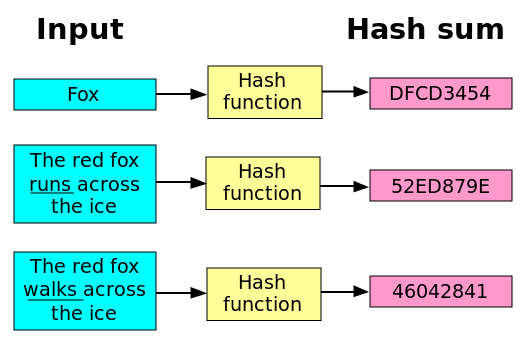
\includegraphics[scale=0.5]{hash_function.png}
\caption{A simplified view of a hash function which represents its input and potential result. The length of the hash sum always remains the same regardless of the input size. Any small change in the input drastically changes the output. TODO redraw image}
\end{figure}


\subsection*{Hash Chains \cite{horne_hash_2011}}

Leslie Lamport \cite{lamport_password_1981} was first to propose the use of hash chains in his paper on a method for secure password authentication over an insecure medium.

\say{A hash chain is a sequence of values derived via consecutive applications of a cryptographic hash function to an initial input. Due to the properties of the hash function, it is relatively easy to calculate successive values in the chain but given a particular value,it is infeasible to determine the previous value} 

As an example, Let $x$ be the initial password a hash chain of length 2 would be $H^{2}(x) = H(H(x))$. So a hash chain of $n$ values is denoted as $H^{n}(x)$ and the $i^{th}$ value in the chain would be computed as $x_{i} = H(x_{i-1})$.

For a given value in the chain $x_{i}$ its computationally infeasible to determine the previous value in the chain $x_{i-1}$.


\section*{Proposed Architecture}

\subsection*{Assumptions}
-Ephemeral client facing servers
-reasoning for ephemeral servers
-netflix \cite{basiri_chaos_2016} 


\begin{figure}[hbtp]
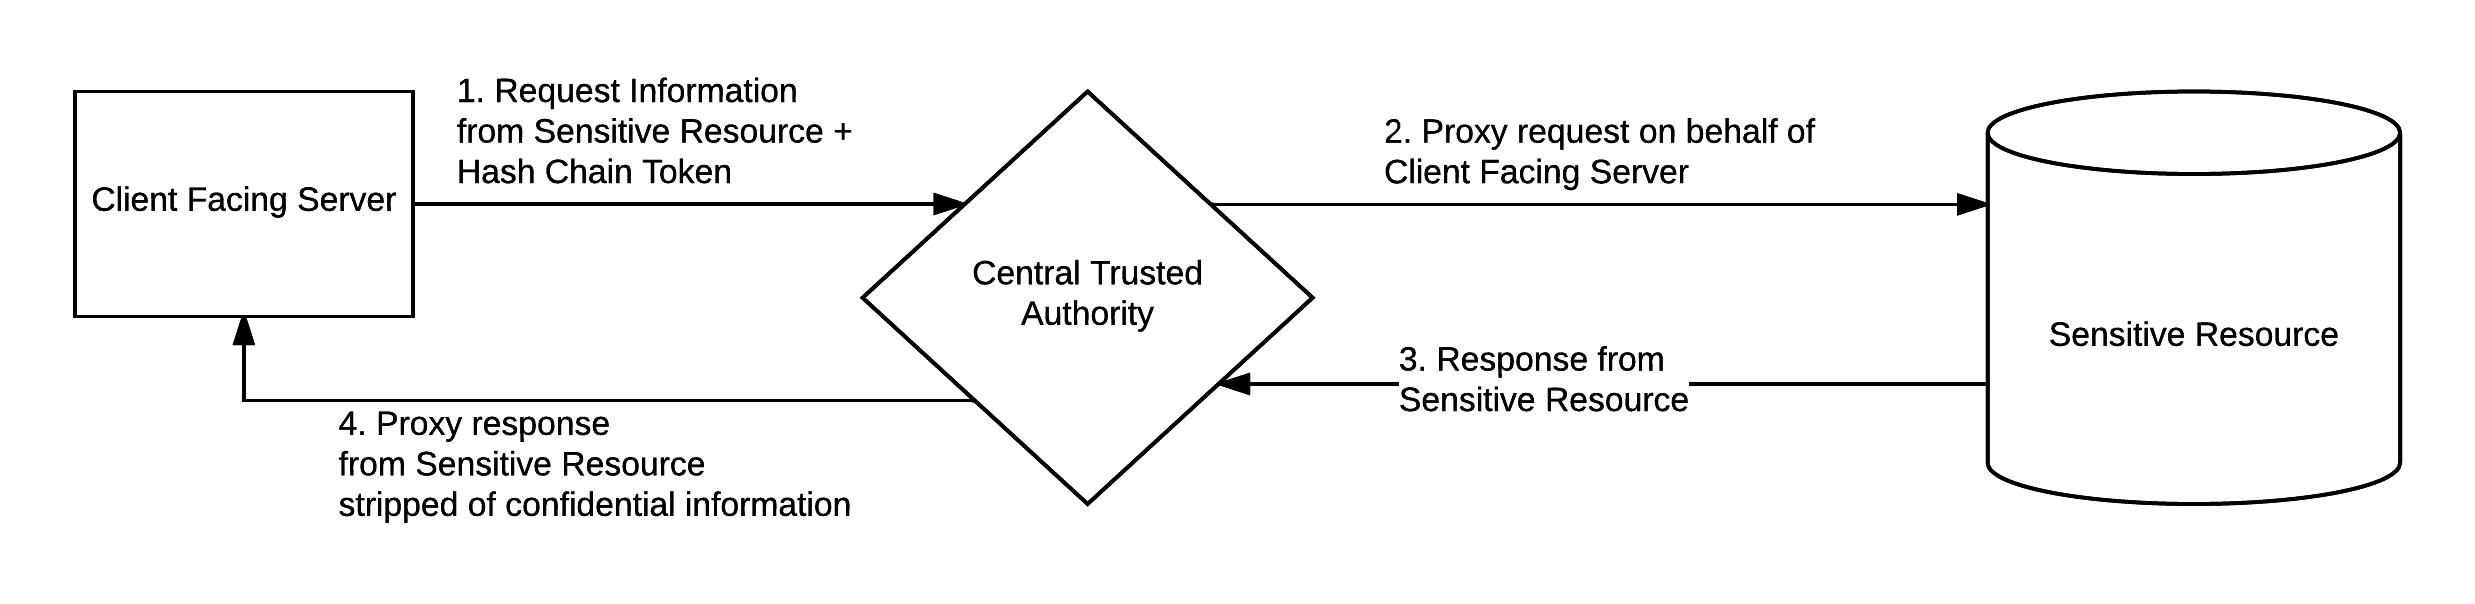
\includegraphics[scale=0.3]{overview_architecture.png}
\caption{Architectural overview of the system. This figure describes the three primary modules involved. The client facing server, The central trusted authority and a sensitive resource.}
\end{figure}



\section*{Performance testing}
\section*{Future work}

- Timed release \cite{chalkias_timed_2006}
- 

\section*{Related work}



\bibliographystyle{plain}
\bibliography{css539_class_see}

\end{document}

